



\documentclass{article}
\usepackage[utf8]{inputenc}
\usepackage{graphicx}
\usepackage{hyperref}
\def\bibsection{\section*{References}}
%
\newcommand*{\fbinv}{\ensuremath{{\rm fb^{-1}}}\xspace}
\newcommand*{\pbinv}{\ensuremath{{\rm pb^{-1}}}\xspace}


\title{WG1 HL-LHC and HE-LHC Executive Summaries}
\author{Patrizia Azzi, Dieter Zeppenfeld, Stephen Farry, Paolo Nason, Alessandro Tricoli }
\date{November 2018}

\begin{document}

\maketitle

%%%%%%%%%%%%%%%%%%%%%%%%%%%%%%%%%%%%%
\section{HL-LHC Executive Summary}
%%%%%%%%%%%%%%%%%%%%%%%%%%%%%%%%%%%%%


%%%%%%%%%%%%%%%%
\subsection{QCD}

{\bf Fig.: Ultimate HL-LHC PDF, e.g. gg parton luminosity}


\begin{figure}
\centering
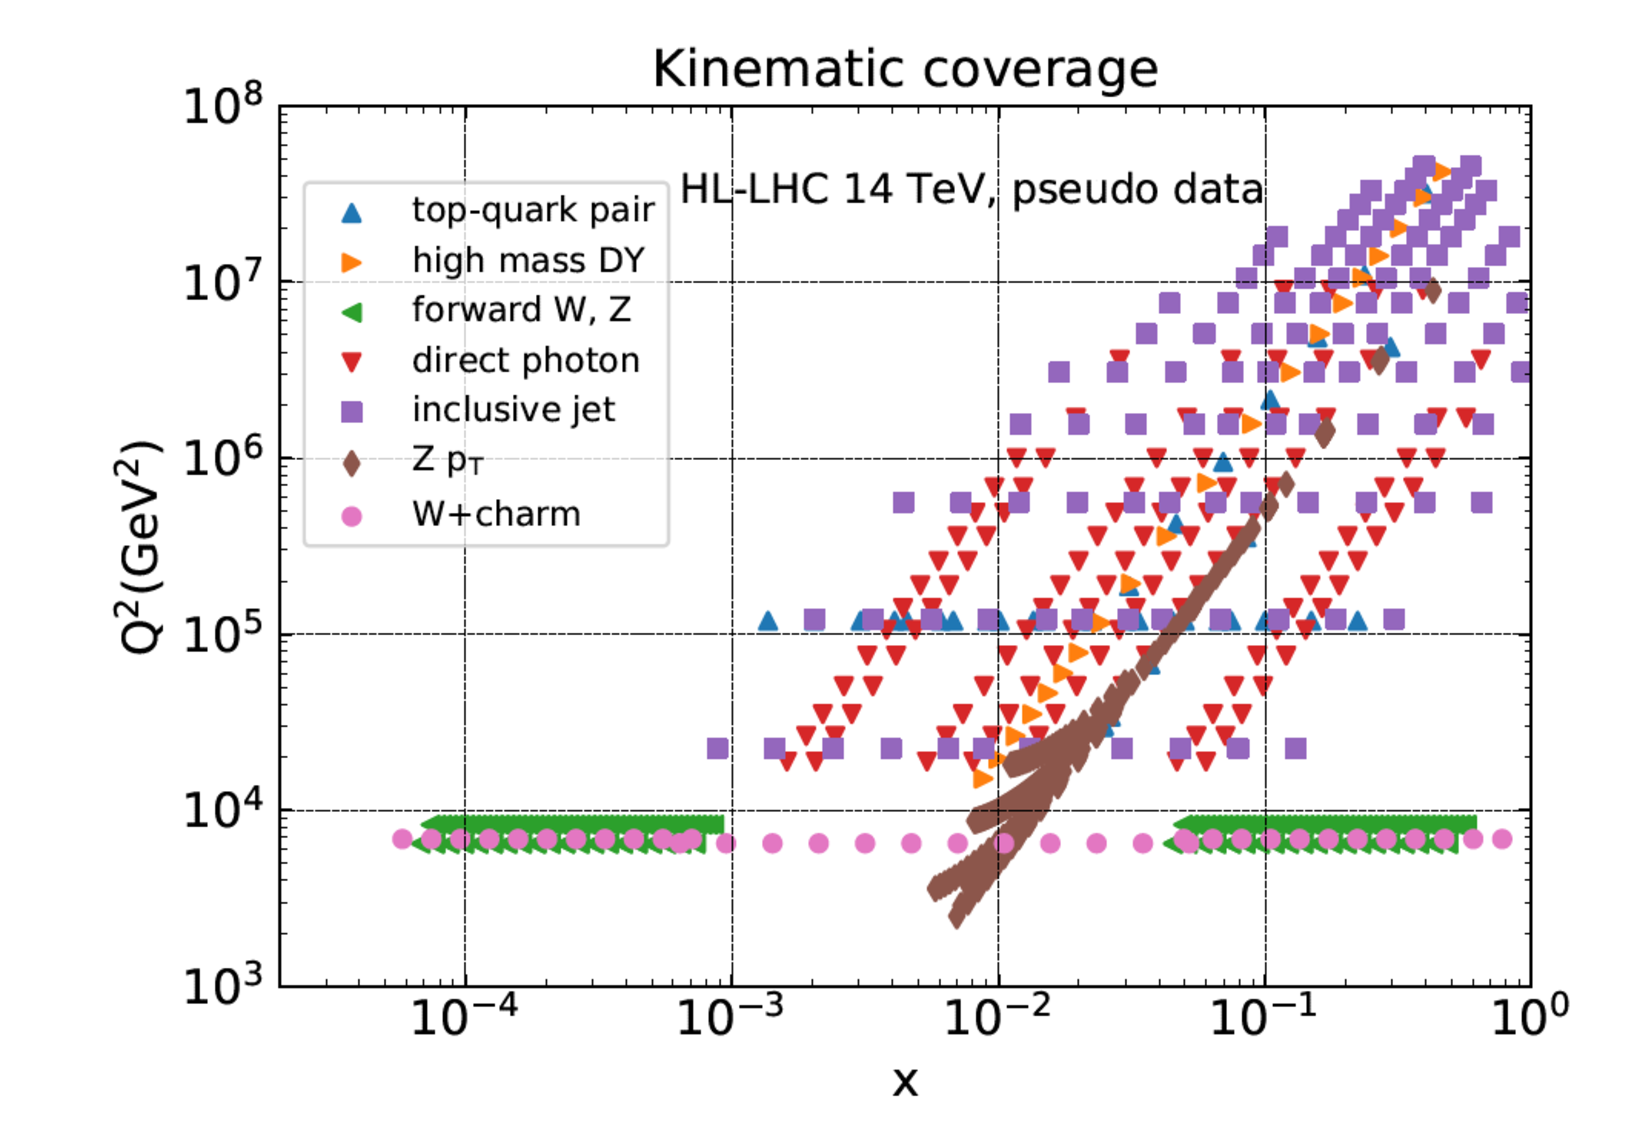
\includegraphics[width=0.7\textwidth]{HLLHC_kinematics.pdf}
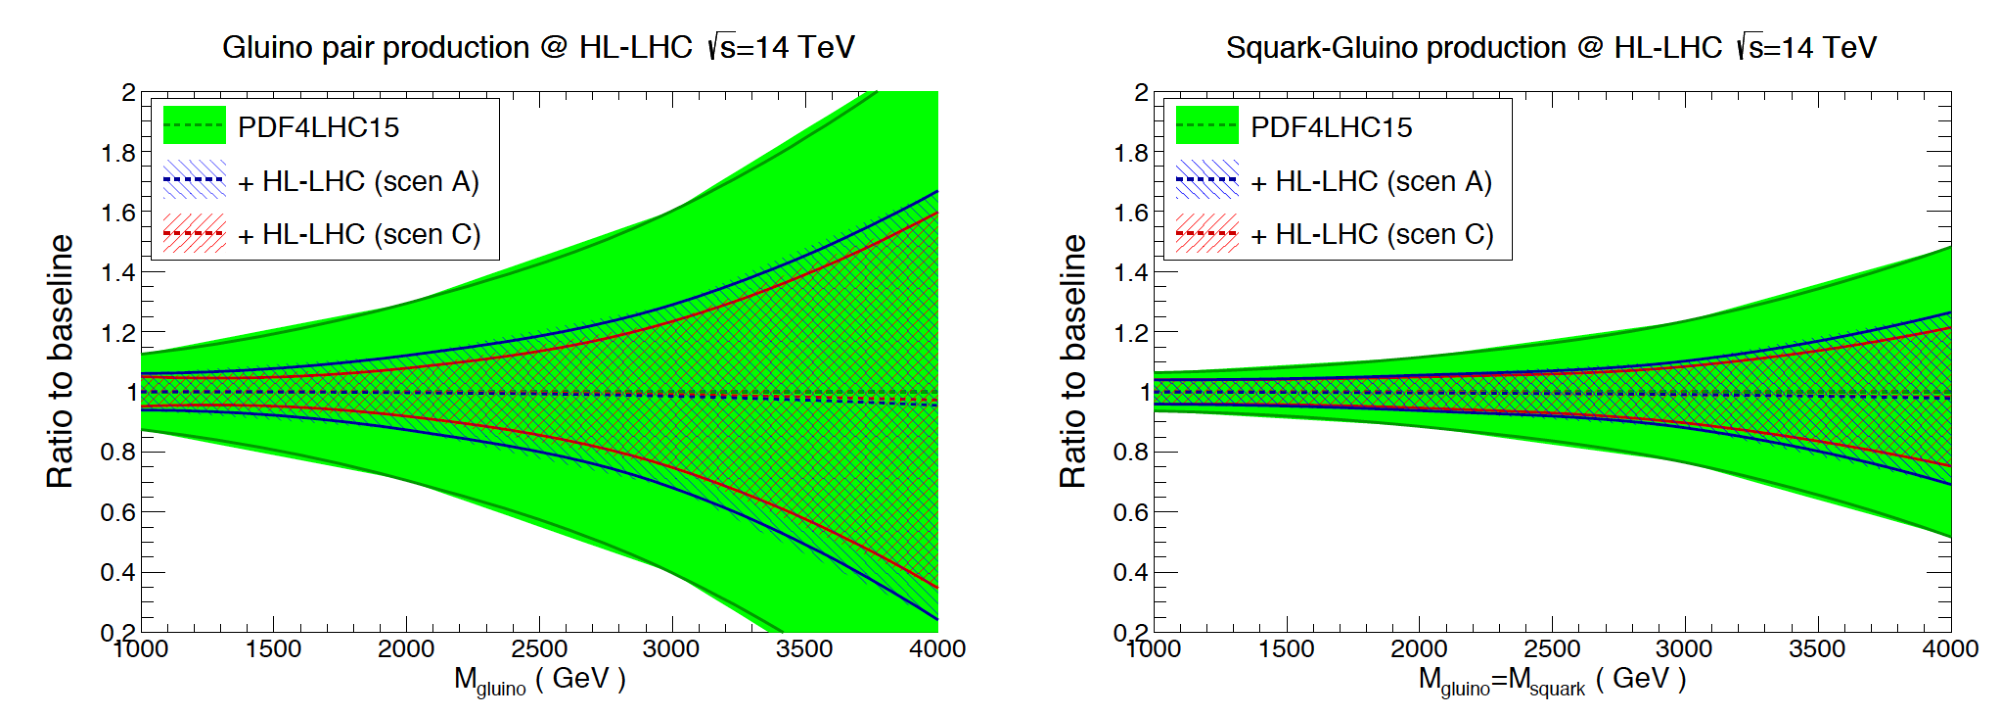
\includegraphics[width=1.0\textwidth]{UltimatePDF_gluino_squark.pdf}
\caption{\label{Fig:HLLHC_kin} (Top) The kinematic coverage in the (x-${\rm Q^2}$) plane of HL-LHC pseudo-data. (Bottom) The cross sections for high-mass supersymmetric particle production at $\sqrt{s}$ = 14 TeV, comparing the predictions of the PDF4LHC15 baseline with those of the HL-LHC PDF sets in the conservative (A) and optimistic (C) scenarios, normalised to the central value of PDF4LHC15. The results corresponding to gluino pair production (left) and squark-gluino production (right). Ref.~\cite{Khalek:2018mdn}}
\end{figure}



\\
{\bf Text: pT reach of jets and photons from ATLAS and CMS}


\\
{\bf Text: MPI - observability of correlations in SS WW MPI analysis}

%%%%%%%%%%%%%%%%
\subsection{EW}

{\bf Fig. : summary plot of experimental cross section precision for several VBS processes, combining results from ATLAS and CMS (ZZ, SS-WW, WZ, Tribosons, semilept WV). For Tribosons we also highlight the expected significance. One bin per analysis with current and projected precisions.}


\begin{table}[htbp]
\caption{Expected yields, cross sections and significances for electroweak processes at 14 TeV $pp$ collisions with 3000~ \fbinv of integrated luminosity.}
\label{tab:yields}
\begin{center}
\begin{tabular}{ | l | c | C | c| c|}
\hline
Process & Yield & $\sigma$ ${\rm [fb^{-1}]}$ & Significance & Precision {\rm $[\%]$} \\
\hline
\hline
$W^\pm W^\pm$ + jj $\to \ell^{\pm}\nu  \ell^{\pm}\nu$ + jj & .... & .... & ... & ...  \\
\hline
$ZZ$ + jj $\to \ell^{\pm}\ell^{\pm}  \ell^{\pm}\ell^{\pm}$ + jj & .... & .... & ...& ...    \\
\hline
$W^\pm Z$ + jj $\to \ell^{\pm}\nu  \ell^{\pm}\ell^{\pm}$ + jj & .... & .... & ...& ...    \\
\hline
$W^\pm V$ + jj $\to \ell^{\pm}\nu$ + jjjj & .... & .... & ... & ...   \\
\hline
\hline 
$W^{\pm} W^{\pm} W^{\mp} \to \ell^{\pm}\nu \ell^{\pm}\nu\ell^{\mp}\nu$ & .... & .... & ... & ...   \\
\hline 
$W^{\pm} W^{\pm} W^{\mp} \to \ell^{\pm}\nu \ell^{\pm}\nu jj$ & .... & .... & ... & ...   \\
\hline
$W^{\pm} W^{\mp} Z \to \ell^{\pm}\nu \ell^{\pm}\nu \ell^+\ell^-$ & .... & .... & ... & ...   \\
\hline 
$W^{\pm} W^{\mp} Z \to \ell^{\pm}\nu jj \ell^+\ell^-$ & .... & .... & ... & ...   \\
\hline
$W^{\pm} Z Z \to \ell^{\pm}\nu \ell^{+}\ell^{-} \ell^{+}\ell^{-}$ & .... & .... & ... & ...   \\
\hline
$W^{\pm} Z Z \to \ell^{\pm}\nu \ell^{+}\ell^{-} \nu\nu$ & .... & .... & ... & ...   \\
\hline 
$W^{\pm} Z Z \to \ell^{\pm}\nu  \ell^{+}\ell^{-} jj$ & .... & .... & ... & ...   \\
\hline 
$W^{\pm} Z Z \to jj \ell^{+}\ell^{-}  \ell^{+}\ell^{-} $ & .... & .... & ... & ...   \\
\hline
\end{tabular}
\end{center}
\end{table}



\\
{\bf Text: Weinberg angle precision at HL-LHC from ATLAS, CMS and LHCb compared current world average}


\\
{\bf Text: W mass precision at HL-LHC with different PDFs, including Ultimate PDF}


\begin{figure}
\centering
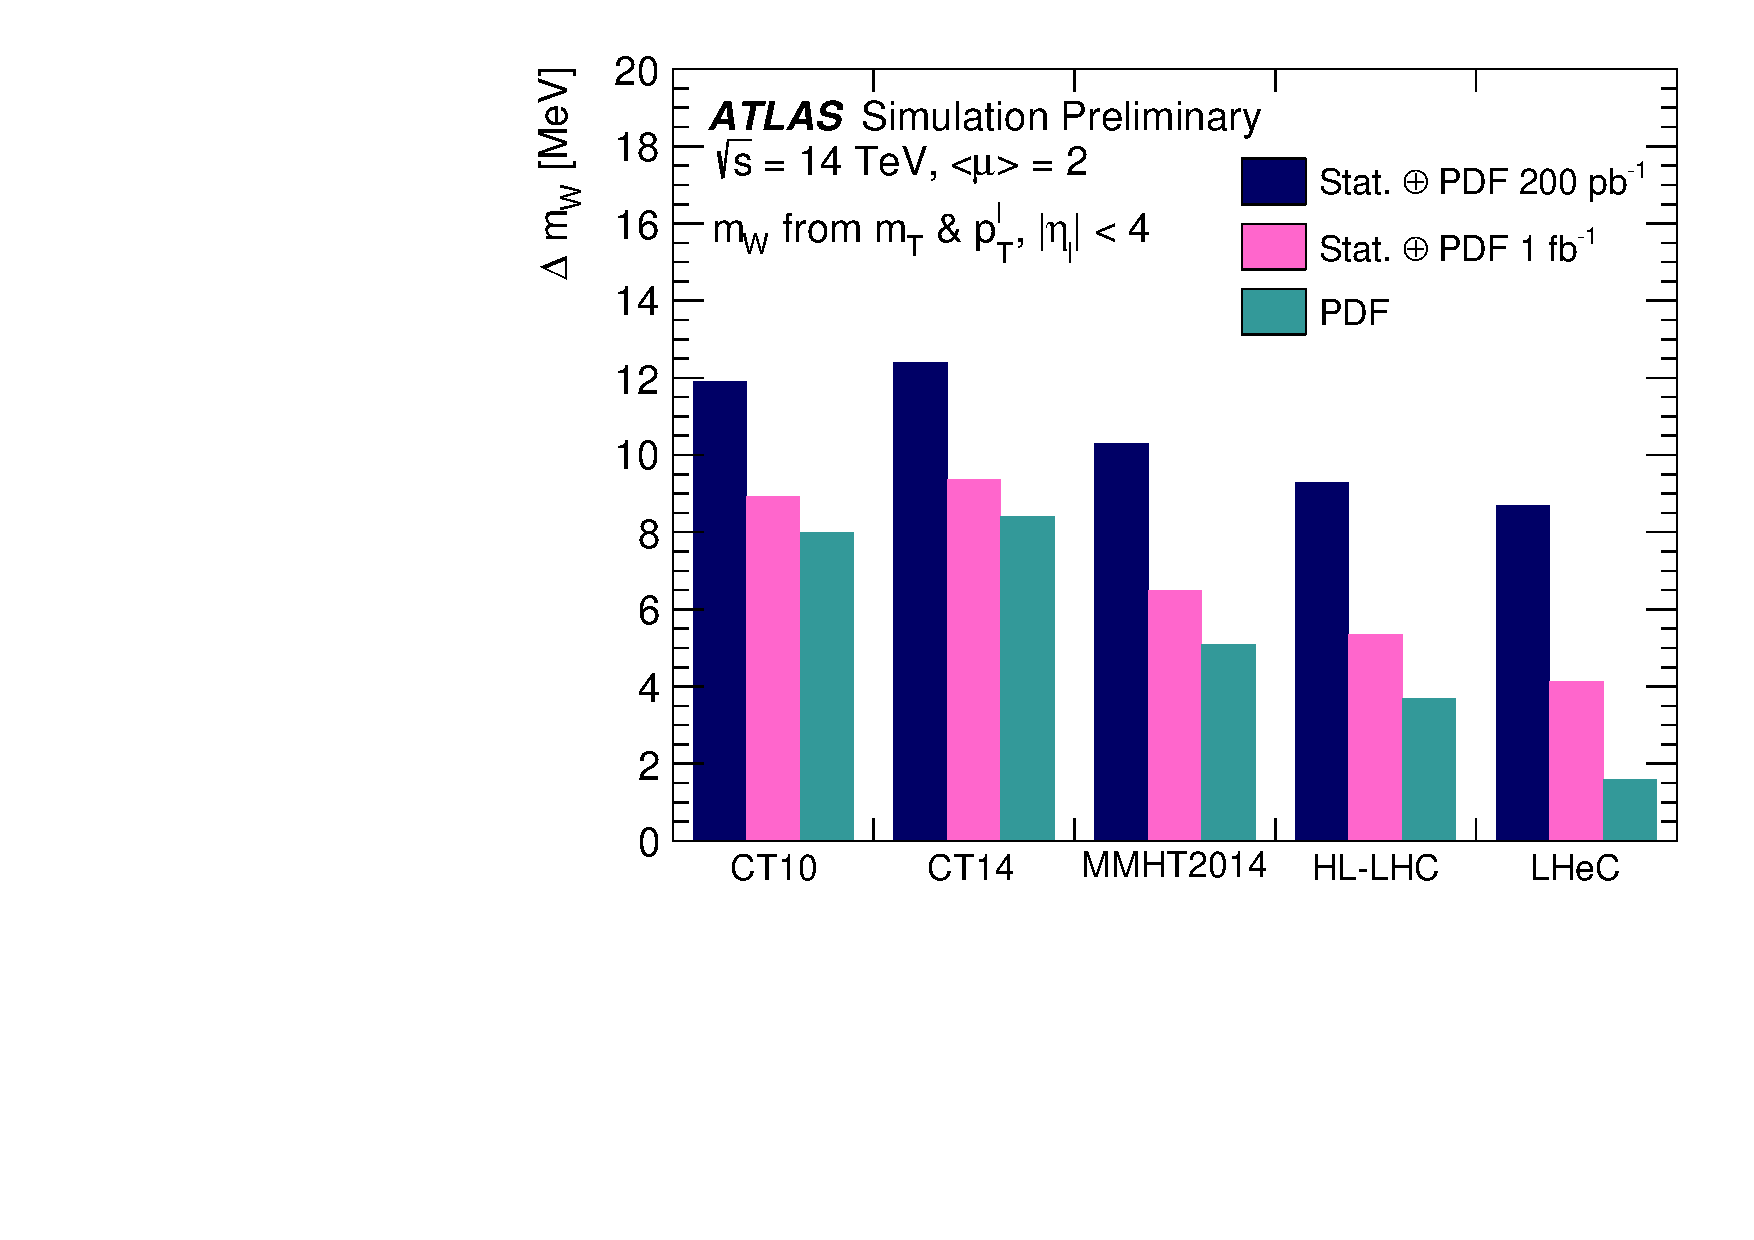
\includegraphics[width=0.9\textwidth]{Wmass_fig_06.pdf}
\caption{\label{Fig:Wmass} The expected statistical and PDF uncertainties on the $W$ mass measurement for different PDF sets, inclusing CT10, CT10, MMHT2014 as well as the predicted Ultimate PDF (HL-LHC) and LHeC PDF,  for the cases of 200 ~\pbinv ~and 1 ~\fbinv~  integrated luminosities, collected at ${\rm \sqrt{s}=14}$ TeV $pp$ collisions at the HL-LHC.}
\end{figure}


%%%%%%%%%%%%%%%%
\subsection{Forward/soft Physics}

{\bf Text: forward electroweak processes, i.e. gamma-induced processes, and reach in EFT limit setting}

%%%%%%%%%%%%%%%%
\subsection{Top}


{\bf Fig. on top mass, combining ATLAS and CMS, for example one bin per method with current and projected errors}


\\
{\bf Fig.: summary of precisions (when necessary significance) of several top process cross section measurements (e.g.4-tops, diff. Xsect tt and single top). One bin per analysis with current and projected precisions.}


\\
{\bf Textual discussion on top physics reach in precision (e.g. differential cross sections) and rare processes}


\\
{\bf Text: FCNC reach compared to current limits (to be shared with other WG's)}

%%%%%%%%%%%%%%%%
\subsection{All}


{\bf Fig.: summary of EFT improvements wrt current limits from Top and EW processes (and Higgs) - to be shared with Higgs group}


\\
{\bf Table: summary of EW fits highlighting increased precision, one row per observable, one column of current and one column for projected precisions}



\clearpage
%%%%%%%%%%%%%%%%%%%%%%%%%%%%%%%%%%%%%
\section{HE-LHC Executive Summary}
%%%%%%%%%%%%%%%%%%%%%%%%%%%%%%%%%%%%%

%%%%%%%%%%%%%%%%
\subsection{QCD}

{\bf Text: pT reach of jets and photons from ATLAS and CMS at 27 TeV wrt 14 TeV}

%%%%%%%%%%%%%%%%
\subsection{EW}

{\bf Table: summary of cross sections at 14 and 27 TeV, one row for 14 TeV one row for 27 TeV and one column per process (or above a kin. cut) }



\\
{\bf Fig.: reach in semilept WV, and aQGC limits wrt HL-LHC}



%%%%%%%%%%%%%%%%
\subsection{Top}

{\bf Table: summary of top cross sections at 14 and 27 TeV, one row for 14 TeV one row for 27 TeV and one column per process (or above a kin. cut) }



\\
{\bf Fig.: FCNC reach compared to HL (shared with other WG's)}


%%%%%%%%%%%%%%%%
\subsection{All}

{\bf Fig.: summary plot of EFT improvements wrt HL limits}

%%%%%%%%%%%%%%%%%%%%%%%%%%%%%%%%%%%%
\bibliographystyle{elsarticle-num}
\bibliography{references}{}
%%%%%%%%%%%%%%%%%%%%%%%%%%%%%%%%%%%%
\end{document}
%%%%%%%%%%%%%%%%%%%%%%%%%%%%%%%%%%%%
